\chapter{\pedpancantitle}
\label{chap:pedpancan}

\section{Abstract}

Circular extrachromosomal DNA (ecDNA) is a driver of oncogene amplification in aggressive cancers. The frequency and diversity of ecDNA has been comprehensively described in many different types of adult cancers and in some selected childhood cancer types, such as neuroblastoma and medulloblastoma. However, the frequency of ecDNA and its association with survival has not been comprehensively analyzed in the spectrum of pediatric cancers. In this study, we used the Amplicon Architect (AA) bioinformatics tool via cloud computing to reconstruct ecDNA sequence structures from Whole Genome Sequencing (WGS) data available in two of the largest publicly accessible pediatric cancer data repositories, the Children's Brain Tumor Network (CBTN) and the St. Jude Cloud cancer genomics platform. In total, we analyzed a retrospective cohort of over 1,600 tumor biopsies from 1,400 different patients, spanning 47 different childhood tumor types. As a result, we identified ecDNA in 15 different pediatric tumor types, with an overall incidence of ecDNA of 10\% in the entire patient cohort. We estimate frequencies of ecDNA in pediatric osteosarcomas (47\%), rhabdomyosarcomas (40\%), retinoblastomas (19\%), ETMRs (all, $n=4$), high-grade gliomas (20\%), and others. Across this cohort, ecDNA was found to be significantly associated with poor survival. Our results show that ecDNA is widely prevalent in pediatric cancers, amplifies known and potentially novel oncogenes, frequently evolves during disease progression, and significantly associates with worse clinical outcomes.

\section{Introduction}

Circular extrachromosomal DNA (ecDNA) has recently emerged as a mechanism for rapid oncogene amplification. Also known as double minutes, ecDNA sequences are typically greater than 1 Mb in size, contain one or more oncogenic sequences, and lack centromeres. ecDNA is subject to non-Mendelian inheritance, leading to unequal segregation of ecDNA during cytokinsesis and consequently intratumoral heterogeneity with every cell division \cite{bafna_2022}. The mechanisms which promote and maintain ecDNA or which suppress or inhibit ecDNA have yet to be fully elucidated. Several methods have emerged for identification of ecDNA, including microscopic examination with FISH and sequencing-based approaches. Algorithmic assembly from short-read whole genome sequencing has arisen as a cost-effective method to identify ecDNA, and has been applied to estimate the prevalence of ecDNA in adult \cite{Kim_2020,pongor_2023,luebeck_2022} and some pediatric cancer types \cite{Koche_2020,Chapman}. However, we are aware of only isolated meta-analyses \cite{gebhart_2005} and case reports describing ecDNA in other pediatric solid tumors including rhabdomyosarcoma, osteosarcoma, retinoblastoma, and others. 

We and others have recently shown that many pediatric cancers harbor unique mutations and driver oncogenes that differ from their adult counterparts \cite{grobner_2018,ma_2018}. However, ecDNA analysis was not included in these pan-cancer studies, in part because computational methods for reconstructing ecDNA from whole-genome sequencing data were not available at the time.  To address this gap, we have now analyzed the frequency of ecDNA in two of the largest publicly available childhood cancer data repositories. The pediatric pan-cancer study presented here identifies childhood cancer types commonly affected by ecDNA, catalogues ecDNA-amplified genes in primary and recurrent tumors, and examines the association between ecDNA and patient survival. In addition to being an indicator of prognosis, ecDNA provides an opportunity for therapies targeting ecDNA-specific properties, but its real-time clinical applicability has yet to be explored. This study seeks to take the first step in this process by highlighting the spectrum of childhood patients who may benefit from future therapies targeting ecDNA. 

\section{Results}

\subsection{ecDNA occurs in at least 15 distinct pediatric tumor types.}

To investigate the prevalence of ecDNA in pediatric tumors, we accessed whole genome sequencing data from two large cloud genomic platforms: St Jude Cloud and Children’s Brain Tumor Network (CBTN). In total, we analyzed a retrospective cohort of \gls{wgs} data of 1670 tumor biopsies from 1481 different patients. Clinical data was available for some patients and included age at diagnosis, sex, survival, tumor tissue site, race/ethnicity, and molecular subgroup for some tumor types. To detect ecDNA, we applied AmpliconArchitect (AA), a tool that detects and reconstructs focal genomic amplifications from whole genome sequencing data \cite{AA}. We then applied AmpliconClassifier, which classifies the reconstructed sequence as ecDNA or a separate noncircular amplification. Amplicons were classified as circular, breakage-fusion-bridge, complex noncyclic, or linear (Fig. \ref{subfig:cloud-workflow-diagram}). 174 ecDNA sequences were detected in tumor tissue of 157 out of 1486 patients (10\%). This cohort spans 47 different tumor types, 15 of which were found to have ecDNA in at least one sample. The frequencies of ecDNA in these 15 cancer types were as follows: \acrfull{ETMR} 4/4 (100\%), \acrfull{PB} 2/4 (50\%), \acrfull{OS} 27/57 (47\%), \acrfull{RMS} 14/35 (40\%), \acrfull{CPC} 1/3 (33\%), \acrfull{NB} 32/106 (30\%), \acrfull{MPNST} 1/4 (25\%), \acrfull{HGG} 32/157 (20\%), \acrfull{RB} 6/32 (19\%), \acrfull{MB} 25/177 (14\%), \acrfull{ACC} 2/21 (10\%), \acrfull{EPN} 2/73 (3\%), \acrfull{CPG} 1/39 (3\%), \acrfull{GG} 1/44 (2\%), and \acrfull{LGG} 1/290 (0.3\%) (Fig. \ref{subfig:pedpancan-piecharts}). ecDNA was significantly associated with tumor type ($\chi^2 = 299.96$, p value $2.2\times10^{-16}$).  ecDNA was not identified in the 32 other tumor types in our cohort.

\begin{figure}[!h]
    \centering
    \begin{subfigure}{\textwidth}
        \centering
        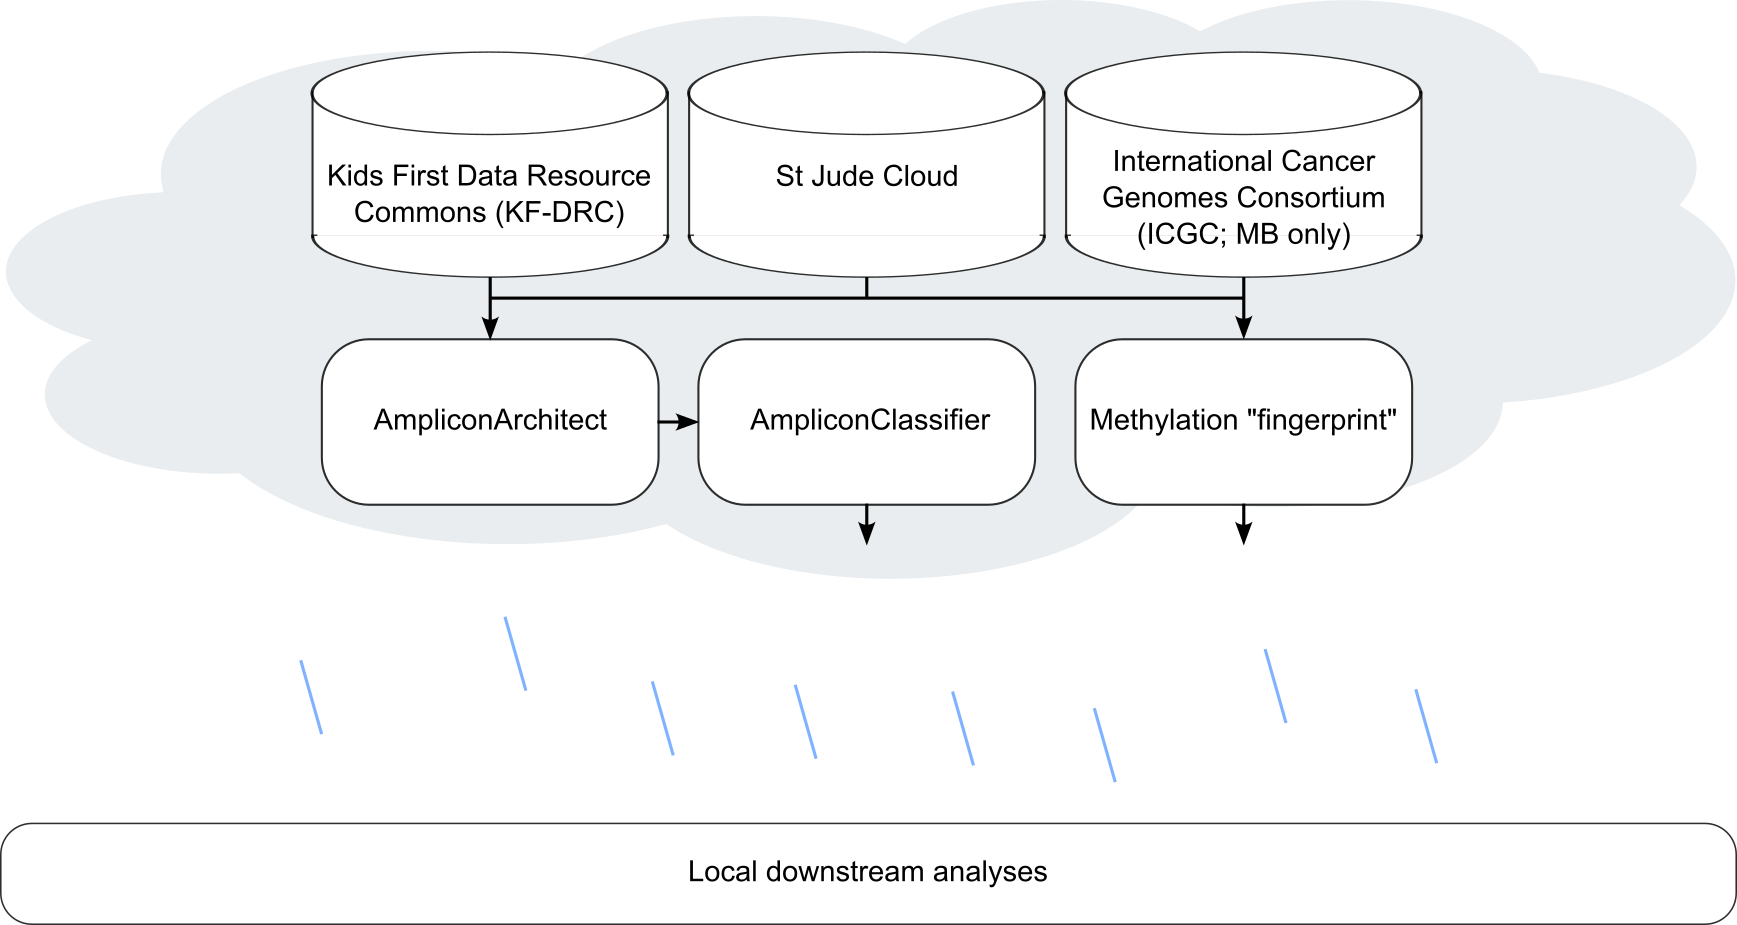
\includegraphics{cloud-workflow-diagram}
        \caption{}
        \label{subfig:cloud-workflow-diagram}
    \end{subfigure}
    \begin{subfigure}{\textwidth}
        \centering
        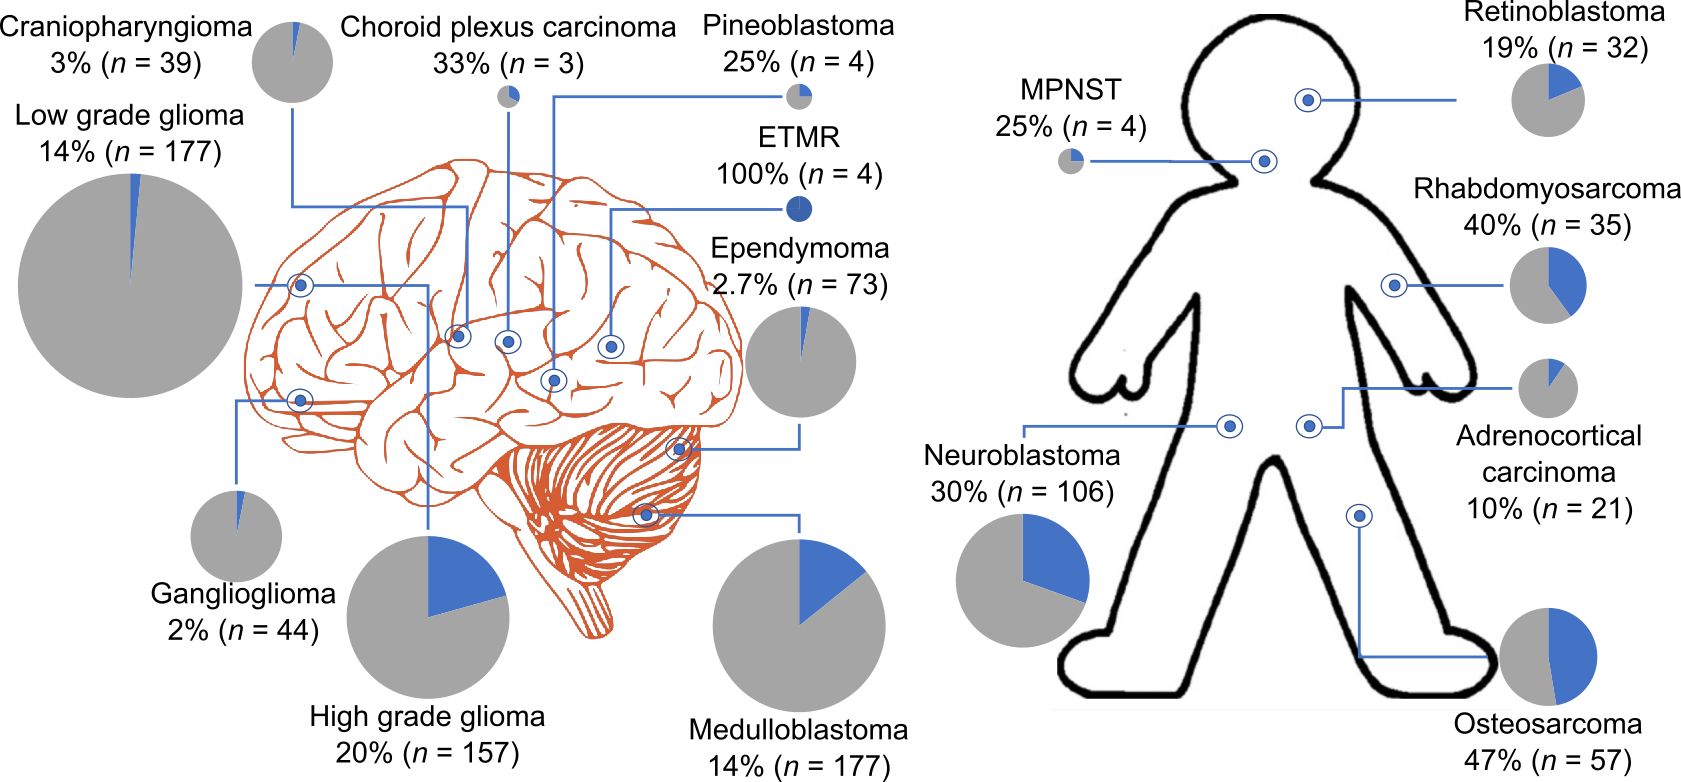
\includegraphics{pedpancan-piecharts}
        \caption{}
        \label{subfig:pedpancan-piecharts}
    \end{subfigure}
    \caption[Frequency of ecDNA sequences across a large restrospective cohort of pediatric tumors.]{\textbf{Frequency of ecDNA sequences across a large restrospective cohort of pediatric tumors.} (\textbf{a}) Analysis workflow diagram of cloud cancer genomics databases of whole genome sequencing data. (\textbf{b}) ecDNA frequencies for select tumor types in this cohort.}
    \label{fig:frequency-pedpancan}
\end{figure}

\subsection{ecDNA status is predictive of 5-year survival across pediatric cancer types.}
To evaluate the relationship between ecDNA and survival across pediatric cancer types, we performed Kaplan-Meier regression analyses across 345 patients for whom clinical metadata were available. Patients with \gls{ecDNA+} tumors had significantly worse five-year overall and progression free survival compared to patients with ecDNA negative tumors (log-rank-test, $p_{OS} < 0.001$, $p_{PFS} < 0.001$) (Fig. \ref{fig:survival-pedpancan}). Individual survival analyses for each tumor type were not significant, attributable to low statistical power. To further substantiate the association between survival and ecDNA status, we performed a Cox regression analysis with ecDNA as the predictor and age and sex as covariates. ecDNA was significantly associated with poor survival ($HR=3.17$, $p = 1.24 \times 10^{-9}$). To determine whether \gls{ecDNA+} tumors had worse outcomes than those with other forms of focal amplification, we compared survival across different classes of amplification: no amplicon, ecDNA, linear, and highly rearranged amplicons). Patients with cyclic amplification had significantly worse overall survival compared to patients with no amplification and linear amplification (\comment{TODO}log-rank test, $p_{OS} < 0.001$). 

\begin{figure}[!h]
    \centering
    \begin{subfigure}{\textwidth}
        \centering
        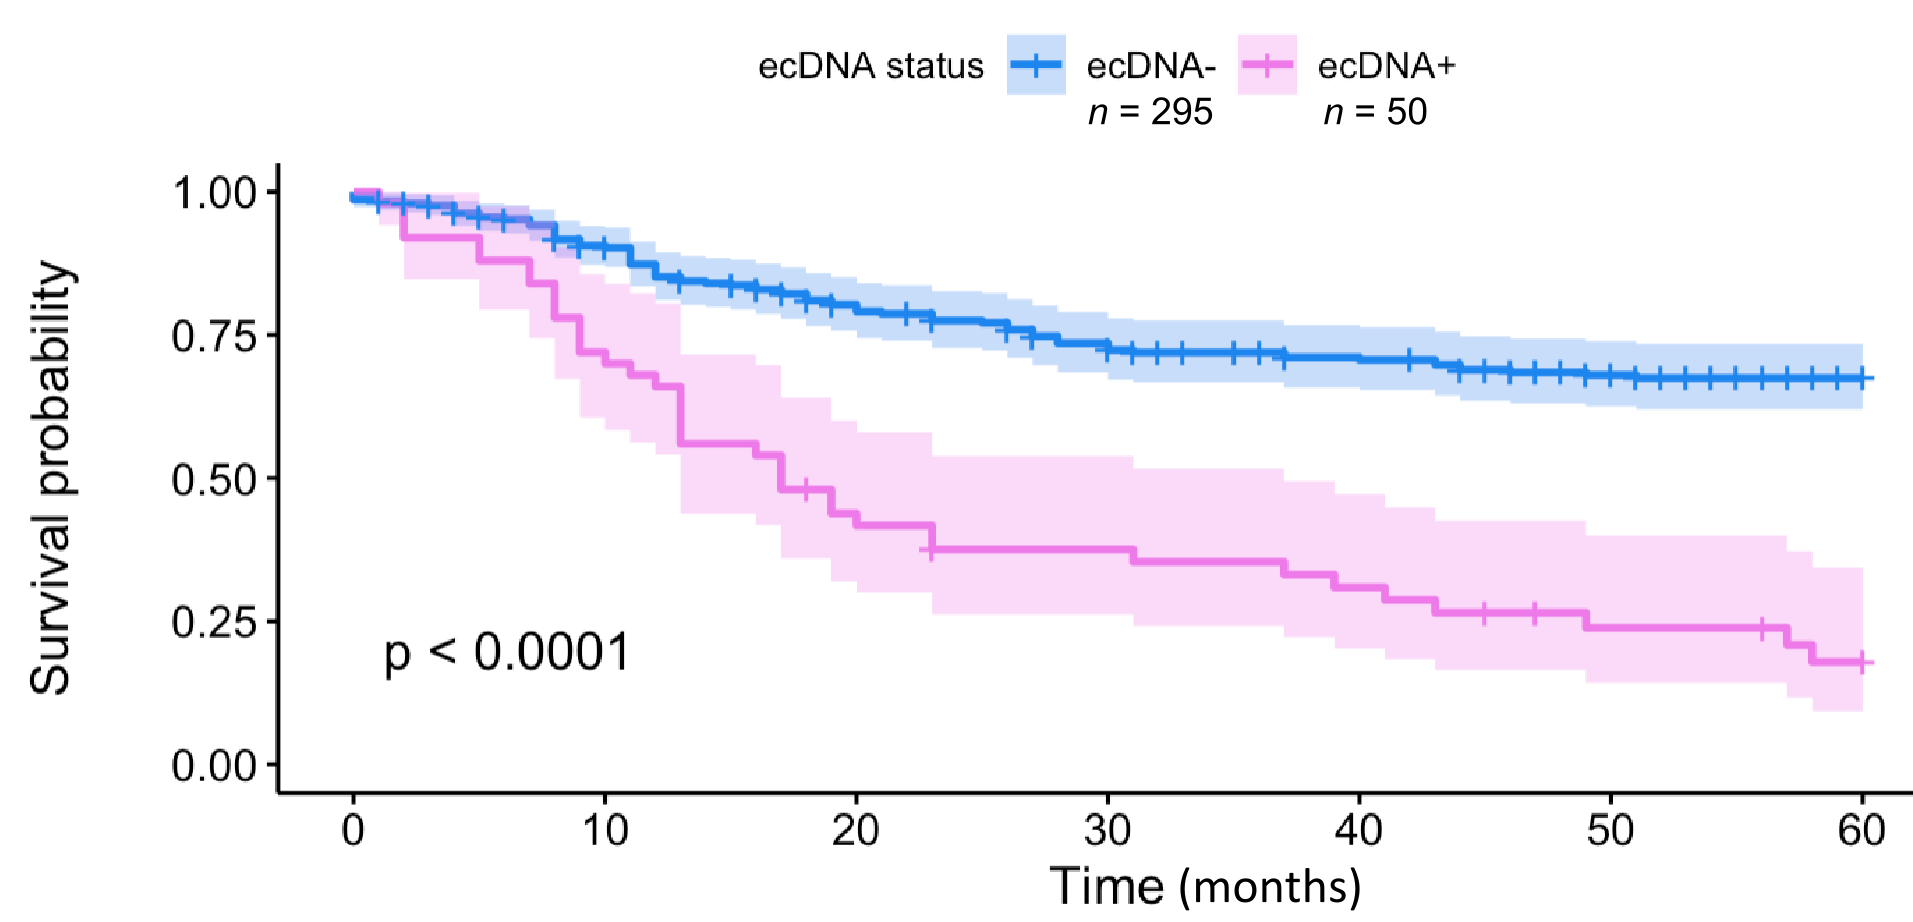
\includegraphics{km-pedpancan}
        \caption{}
        \label{subfig:km-pedpancan}
    \end{subfigure}
    \begin{subfigure}{\textwidth}
        \centering
        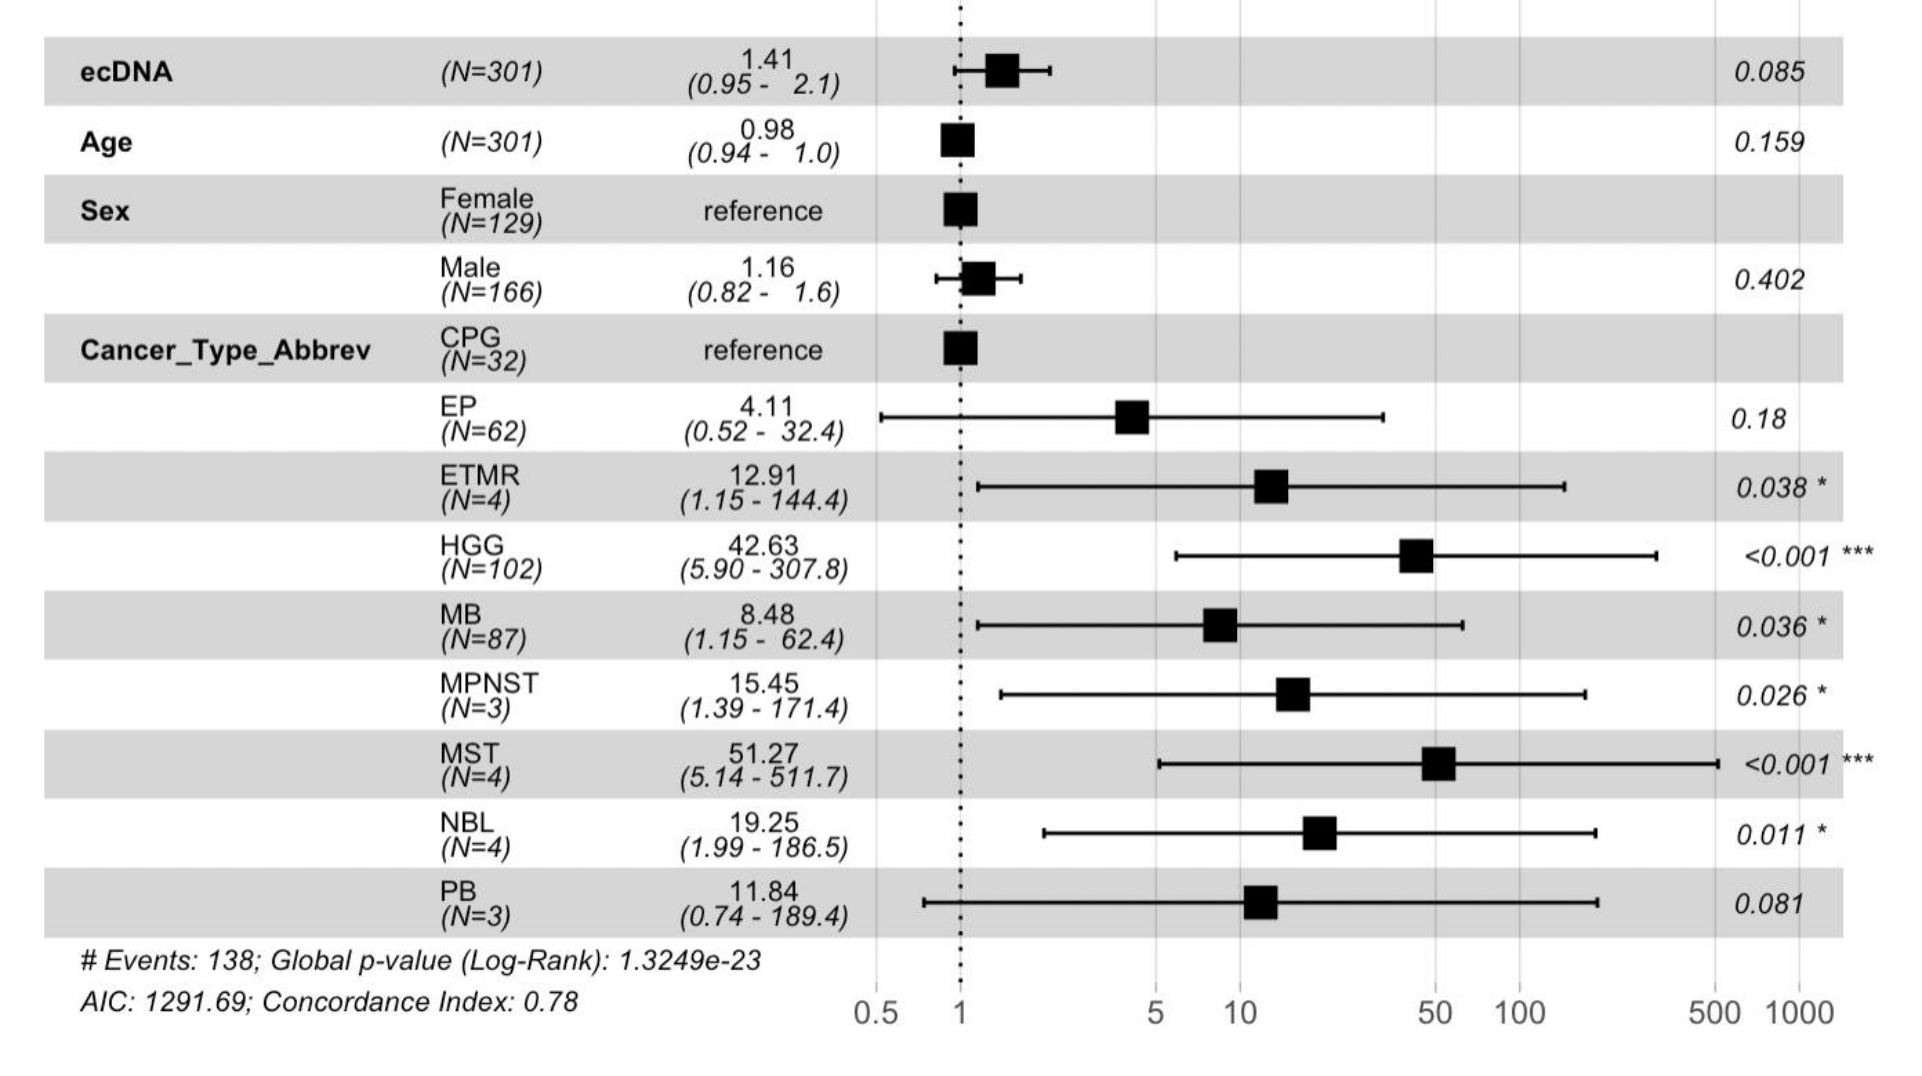
\includegraphics{cph-pedpancan}
        \caption{}
        \label{subfig:cph-pedpancan}
    \end{subfigure}
    \caption[Survival analysis of a retrospective cohort of 345 patients across \textit{n} pediatric tumor types.]{\textbf{Survival analysis of a retrospective cohort of 345 patients across \textit{n} tumor types.} (\textbf{a}) Kaplan-Meier curves indicating 5-year overall survival for ecDNA+ and ecDNA- patients. (\textbf{b}) Cox Proportional Hazards regression coefficients indicating log relative hazards for age, sex, ecDNA status and tumor type.}
    \label{fig:survival-pedpancan}
    % TODO Update n of patients and tumor types in this analysis
\end{figure}

Molecular subgroup annotations were available for 108 for \gls{HGG} tumors, facilitating comparison of the effect size of ecDNA on survival relative to other molecular determinants of risk. The most current subgrouping of \gls{HGG} includes classification into \gls{H3K27mut}, \gls{H3G34mut}, \gls{IDHmut} and \gls{H3/IDHwt} tumors \cite{mackay_2017}. ecDNA was distributed across these subgroups as follows: \gls{H3K27mut} (14/56, 25\%), \gls{H3G34mut} (0/4, 0\%), \gls{IDHmut} (2/6, 33\%), and \gls{H3/IDHwt} (11/42, 26\%). Cox regression indicates that molecular subgroup, especially H3K27 mutation status, is a major determinant of patient outcome ($HR = 4.39$, $p < 0.001$), consistent with previous results \cite{mackay_2017}. This model estimates a modest but insignificant effect of ecDNA on patient survival ($HR = 1.13$, $p = 0.6$, Fig. \ref{fig:survival-hgg}).

\begin{figure}[!h]
    \centering
    \begin{subfigure}{\textwidth}
        \centering
        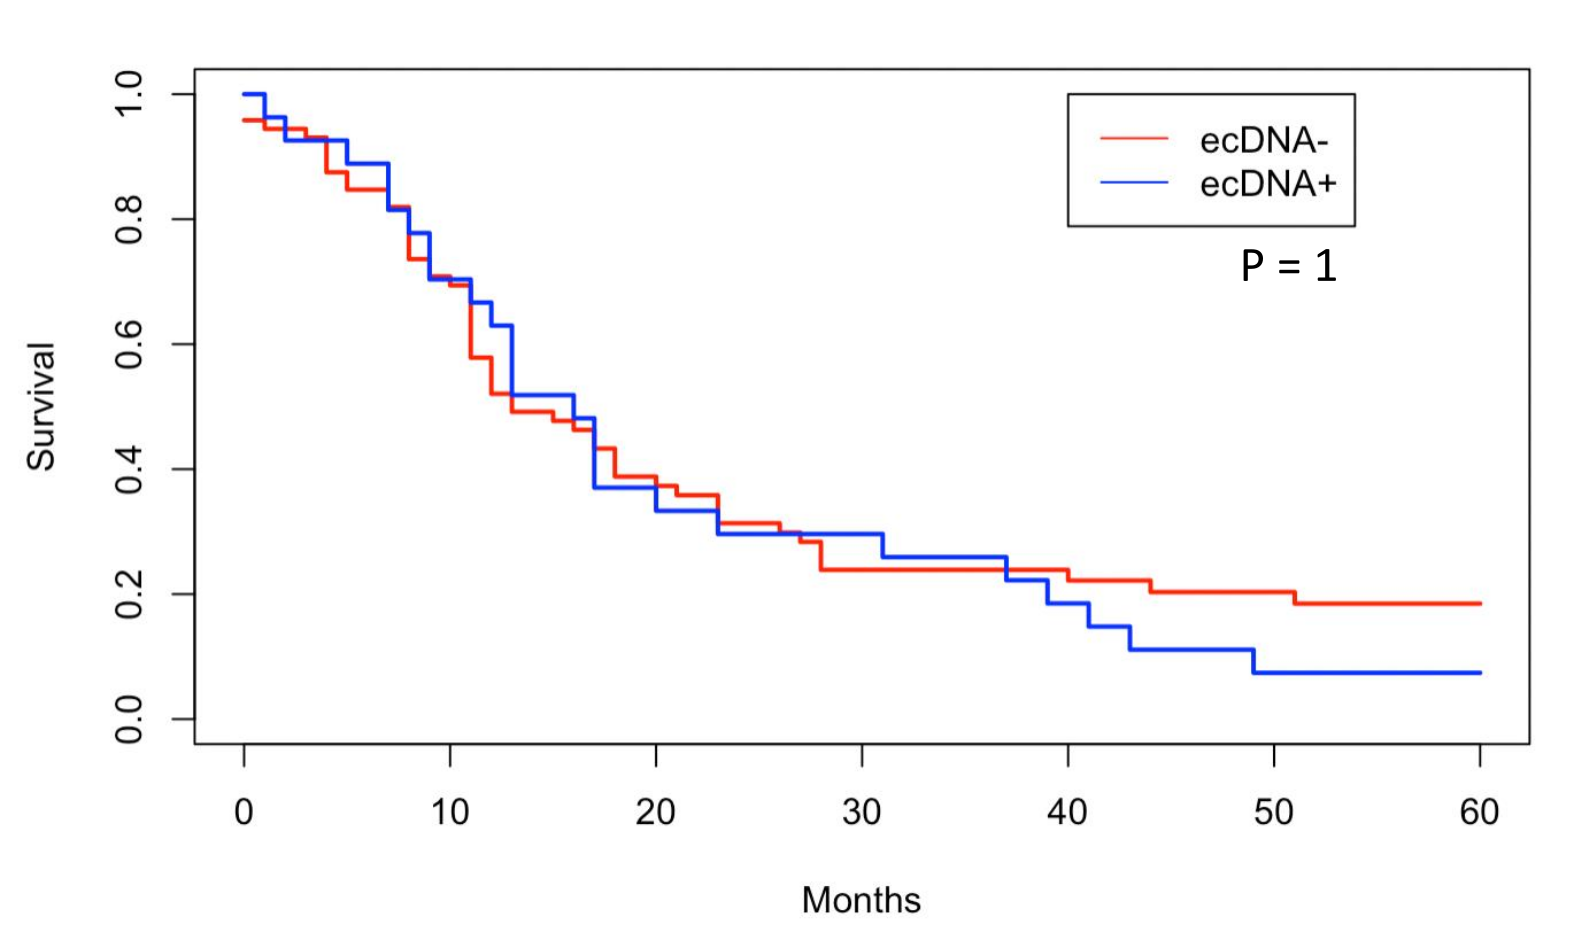
\includegraphics{km-hgg}
        \caption{}
        \label{subfig:km-hgg}
    \end{subfigure}
    \begin{subfigure}{\textwidth}
        \centering
        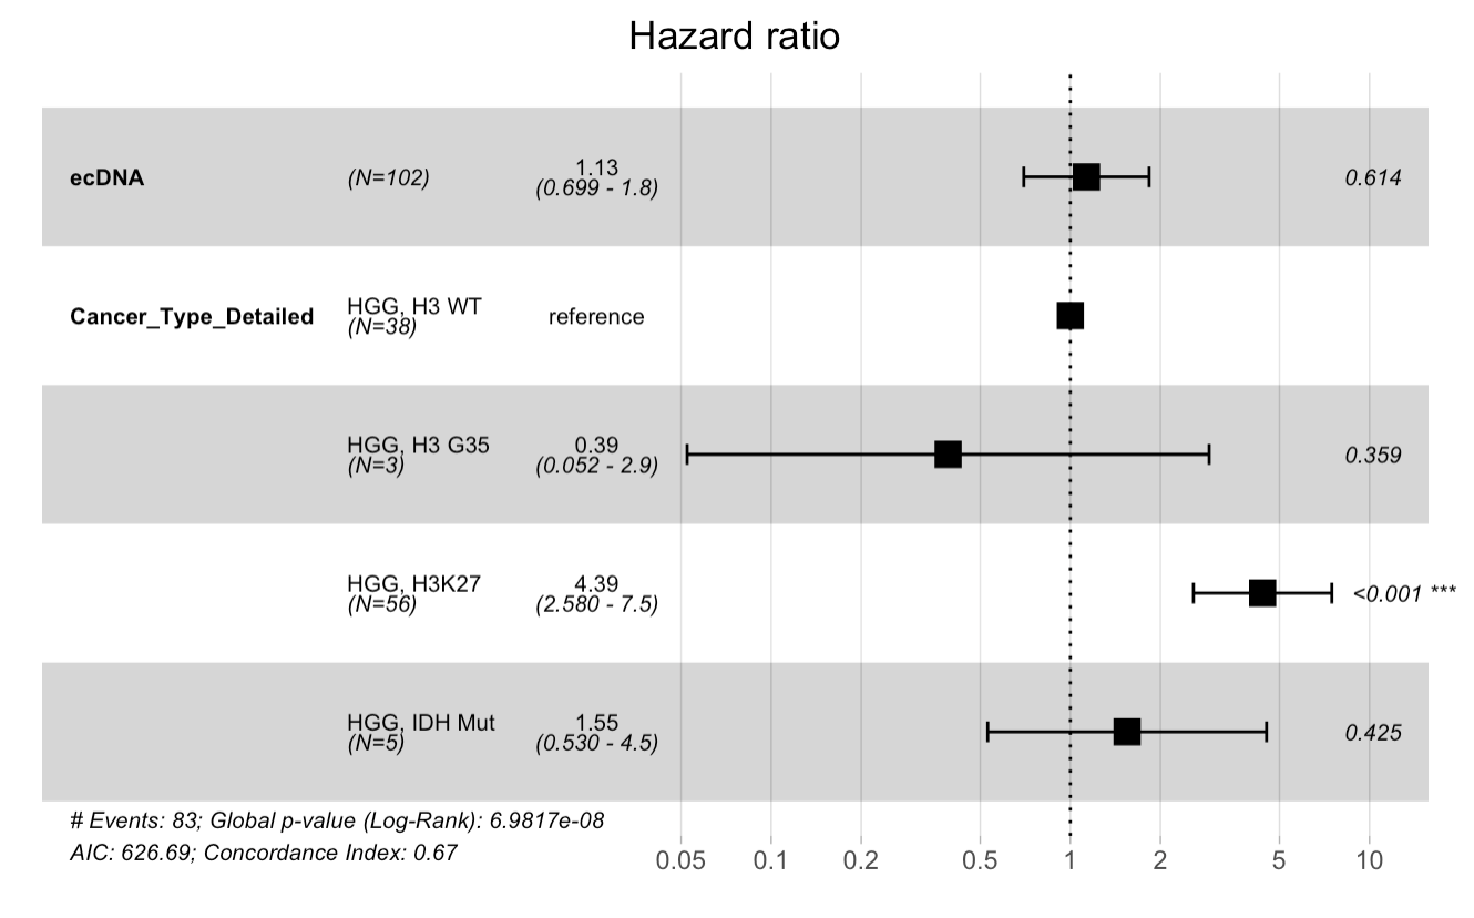
\includegraphics{cph-hgg}
        \caption{}
        \label{subfig:cph-hgg}
    \end{subfigure}
    \caption[Survival analysis of a retrospective cohort of 108 pediatric \gls{HGG} patients.]{\textbf{Survival analysis of a retrospective cohort of 108 pediatric \gls{HGG} patients.} (\textbf{a}) Kaplan-Meier curves indicating 5-year overall survival for ecDNA+ and ecDNA- patients. (\textbf{b}) Cox Proportional Hazards regression coefficients indicating log relative hazards for ecDNA status and tumor type.}
    \label{fig:survival-hgg}
\end{figure}

\subsection{ecDNA most commonly amplifies \textit{MYCN} in neuroblastoma.} 
\label{NB}
The genomic landscape of ecDNA in neuroblastoma has been thoroughly described \cite{Koche_2020, yi_2022}, and the distribution of ecDNA in this neuroblastoma patient cohort is largely consistent with previous observations. We identify circular ecDNA amplification in 32 out of 106 neuroblastomas (30\%). ecDNA amplification was almost exclusively detected at the \textit{MYCN} oncogene locus (30 out of 31, 97\%). 

\subsection{ecDNA amplifies C19MC-\textit{TTYH1} fusions in \acrlong{ETMR}.} Nine out of ten \gls{ETMR} tumors harbor oncogenic amplification and fusion of \textit{TTYH1} with the C19MC microRNA cluster \cite{li_2009, lambo_2019}. Our cohort includes 4 \gls{ETMR} tumors, all \textit{TTYH1}-C19MC amplified on ecDNA. One of these also had noncircular \textit{MYCN} amplification, suggesting a secondary driver.

\subsection{\textit{MYC} amplification occurs on ecDNA in \acrlong{PB}} \Glspl{PB} comprise five molecular subgroups, including a subgroup harboring recurrent amplification of \textit{MYC} \cite{li_2020}. We identify 2 ecDNA sequences in 4 \gls{PB} patient tumors, one amplifying \textit{MYC} and the other the C19MC cluster canonically amplified in \gls{ETMR}. It remains unknown whether the C19MC-amplified \gls{PB} shares other molecular or clinical features with \gls{ETMR} tumors.

\subsection{ecDNA amplifies diverse \acrlong{RMS} oncogenes including \textit{FOXO1}-\textit{PAX7} fusions.}
ecDNA has been described in \gls{RMS} case reports since 1971 \cite{granberg_1971, steilen-gimbel_1996, meddeb_1996, gil-benso_2003, mysorekar_2008}. A review of case literature  \cite{gebhart_2005} identifies ecDNA in 15\% of human rhabdomyosarcomas ($n=84$). We identify ecDNA in \gls{wgs} of 14 out of 35 \gls{RMS} tumors (40\%). Amplified oncogenes were \textit{SOX21} (putative, $n=3$), \textit{MYCN} ($n=2$), \textit{FGFR1} (2), \textit{MDM2} (2), \textit{NSD3} (2), and \textit{FOXO1}-\textit{PAX7} fusion (2). One ecDNA  sequence did not contain any known oncogenes. Both \textit{MYCN} amplification  \cite{williamson_2005} and \textit{FOXO1} fusion \cite{missiaglia_2012} are prognostic indicators of poor \gls{RMS} patient outcomes; however it remains unknown whether properties of ecDNA contribute to these outcomes.

\subsection{Half of focal amplifications in \acrlong{OS} are circular.}
Osteosarcomas have among the highest rates of structural variation among pediatric cancer types \cite{pcgp}, and over 90\% carry inactivating mutations of the p53 pathway \cite{chen_2014}. A previous case literature review reported ecDNA in 21\% of OS tumors ($n=146$) \cite{gebhart_2005}. We detect ecDNA in \gls{wgs} of 27 out of 57 OS patient tumors (47\%). The genomic distribution of ecDNA amplifications largely reflected the known regions of recurrent focal amplification in OS, including \textit{MYC} ($n=4$ patients) \textit{RUNX2} ($n=3$), and chr17p11.2-p12 ($n=6$). chr17p11.2-p12 contains unstable low-copy repetitive sequences which are amplified in pediatric  \gls{OS} \cite{van_dartel_2002} and \gls{MB} \cite{Chapman}, and adult \gls{HGG} \cite{van_dartel_2003}, \gls{MM} \cite{fabris_2007}, \gls{LMS} and \gls{MFH} \cite{kaur_2007}. Genes with putative oncogenic roles within this region include \textit{PMP22}, \textit{COPS3}, \textit{TOP3A}, \textit{MAPK7}, and \textit{MAP2K4} \cite{van_dartel_2002}. 

\subsection{ecDNA amplifies the known landscape of focal amplifications in pediatric \acrfull{HGG}}
Among adult patient tumors, ecDNA occurs most frequently in glioblastomas \cite{Kim_2020}. Reconstruction of circular ecDNA from \gls{wgs} of a large cohort of adult glioblastomas previously identified recurrent ecDNA amplification of \textit{EGFR}, \textit{MDM2}, \textit{CDK4} and \textit{MYCN} in descending frequency \cite{sanborn_2013}. In a large cohort of pediatric \gls{HGG}, also included in our dataset, focal amplification was previously reported of oncogenes \textit{PDGFRA}, \textit{MET}, \textit{EGFR}, \textit{MYC}, \textit{MYCN}, Cyclin D family members \textit{CCND1/2/3}, and Cyclin D-dependent kinases \textit{CDK4/6}. The circular structure of one of these amplicons (\textit{EGFR}) was subsequently comprehensively described at diagnosis and relapse \cite{xu_2019}. We identify ecDNA in 32 of 157 \glspl{HGG} (20\%). Circular amplicons included all of the oncogenes previously described as amplified in this cohort, establishing  circular ecDNA as a frequent form of oncogenic amplification in \gls{HGG}.
% Fusion genes?

\subsection{\textit{MYCN} amplification occurs on ecDNA in a high-risk subset of ependymomas.}
Amplification of the \textit{MYCN} oncogene defines a subset of \gls{EPN} tumors with exceptionally poor prognoses \cite{ghasemi_2019}. Given that in neuroblastoma, \textit{MYCN} is almost exclusively amplified on ecDNA and confers poor prognosis, we investigated whether \textit{MYCN} amplification can occur on ecDNA in \gls{EPN}. We identify 2 ecDNA sequences across 73 \gls{EPN} tumors. This cohort included a single patient with \textit{MYCN}-amplified spinal \gls{EPN}, where \textit{MYCN} was amplified on circular ecDNA in both primary and progressive tumors. The other ecDNA comprised amplification of segments of chr13q33, which to our knowledge has not been described in \gls{EPN}, but is amplified in other cancers \cite{knuutila_1998}. Genes with putative oncogenic roles within this amplicon include \textit{ITGB1L1} \cite{wang_2022}, \textit{ZIC2} \cite{liu_2022} and \textit{ZIC5} \cite{tan_2022, song_2022}.

\subsection{ecDNA amplifies \textit{RB1} fusion genes in RB.}
\Gls{RB} is generally distinguished by early biallelic inactivation of the \textit{RB1} tumor suppressor gene followed by subsequent driver mutations, but 3\% of non-hereditary \glspl{RB} carry wild-type \textit{RB1} and high-copy amplification of \textit{MYCN} \cite{rushlow_2013}. Other high-copy focal amplifications previously reported in \gls{RB} include \textit{MDM4} and co-amplification of \textit{OTX2} and \textit{AKT1} \cite{sakai_1985}. Given that \textit{MYCN}-amplified \gls{RB} bears histological resemblence to \gls{NB} \cite{rushlow_2013}, and that \textit{MYCN} amplifications occur almost exclusively on ecDNA in \gls{NB} (see \ref{NB}), we hypothesized that \textit{MYCN} amplification in \gls{RB} also occurs on ecDNA. We identify circular ecDNA in 6 of 32 \gls{RB} patient tumors. Two of these harbored \textit{MYCN} amplification on ecDNA, out of 3 total \textit{MYCN}-amplified \gls{RB} tumors. Other notable oncogenes amplified on ecDNA included \textit{OTX2} ($n=1$), \textit{SMARCA5} ($n=1$), and putative \textit{RB1} fusion genes ($n=2$): \textit{RB1-THSD1} and \textit{RB1-LHFPL6}. Both amplicons fused the 5' end of \textit{RB1} to the 3' end of the partner gene. No RNA-seq data were available to confirm expression of the putative fusion gene product. However, the recurrent high-copy amplification of truncated \textit{RB1}, and the absence of a high-confidence oncogene on either amplicon, make it tempting to speculate that the \textit{RB1} fusion products provide some other selective advantage beyond \textit{RB1} inactivation.

% \subsection{ecDNA was not detected in low-risk pediatric solid tumor types.}
% ecDNA was not detected in WT, PCP, etc. 
% ecDNA was detected in less than 5% of ...
% any observations about trends (could also be discussion).

\section{Discussion}

Our survey of circular ecDNA across a large cohort of many different pediatric tumor types reveals that ecDNA is most frequent in high-risk malignant tumors, and largely absent from low-risk or benign tumors. For example, ecDNA was detected in one in five high-grade gliomas, but only one in 290 low-grade gliomas. The landscape of ecDNA-amplified genes largely reflects previously-known landscapes of gene amplification, indicating that the oncogenic sequence is not only amplified, but circular and acentric as well. Similarly to a recent result in adult cancers, patients with tumors harboring circular acentric amplifications had worse five-year survival than patients with other forms of amplification.

\par Recurrently ecDNA-amplified genomic loci in other pediatric tumor types span the spectrum of known oncogenes in pediatric cancer: \textit{MYC} family proto-oncogenes, cyclin-dependent kinases, C19MC, growth factor receptors, and others. We highlight unanswered questions around a few recurrent ecDNA loci as promising areas of future study.

\par The chromosomal band chr17p11.2-p12 is ecDNA-amplified in 6 \gls{OS} and 1 \gls{MB} tumors in our cohort, and its amplification has been described in various adult cancers. Copy number variation in this region has also been shown to cause the childhood developmental disorders \gls{SMS} (deletion) \cite{gropman_2006} and \gls{CMT1A} (tandem duplication) \cite{thomas_1997}. The mechanism underlying both syndromes is believed to be unequal crossing over due to homologous recombination between flanking repeat gene clusters \cite{potocki_2000}. It remains to be shown whether the ecDNA amplifications at that locus arise by a similar mechanism.

\section{Methods}

\subsection{Pediatric Tumor WGS}

\subsubsection{CBTN – Children’s Brain Tumor Network (992 biosamples from 831 patients)} WGS of a variety of pediatric tumor biopsies were identified using the Gabriella Miller Kids First Data Resource center portal (\url{https://portal.kidsfirstdrc.org/}). Patients were originally sequenced as part of the Pediatric Brain Tumor Atlas (PBTA) (\url{https://cbtn.org/pediatric-brain-tumor-atlas}). WGS data were preprocessed and aligned to human reference genome hg38 using the Kids First harmonized WGS pipeline (\url{https://github.com/kids-first/kf-somatic-workflow}) and subsequently analyzed using Cavatica (\url{https://cavatica.sbgenomics.com/}), on the cloud genomic analysis platform for Kids First genomic data. Docker containers containing fingerprint and AmpliconArchitect software were installed on the Cavatica cloud genomics platform (see section \ref{4-classification}).

\subsubsection{St. Jude – St Jude Cloud Repository (678 biosamples from 655 patients)} WGS of pediatric tumor biopsies were identified using the St Jude Cloud data portal. Patients were sequenced as part of the \gls{pcgp} and \gls{rtcg}. AmpliconArchitect software was installed on the SJ Cloud platform (see section \ref{4-classification}). 

\subsection{ecDNA detection and classification from bulk WGS}
\label{4-classification}
To detect ecDNA, all samples in the WGS cohort were analyzed using AmpliconArchitect v1.2 \cite{AA} and AmpliconClassifier v0.4.4 \cite{Kim_2020}. Briefly, the AmpliconArchitect algorithm was performed as follows. Copy number segmentation and estimation were performed using CNVkit v0.9.667 \cite{cnvkit}. Segments with copy number $ CN \geq 4$ were extracted using PrepareAA (April 2020 update) as “seed” regions. For each seed, AmpliconArchitect searches the region and nearby loci for discordant read pairs indicative of genomic structural rearrangement. Genomic segments are defined based on boundaries formed by genomic breakpoint locations (identified by discordant reads) and by modulations in genomic copy number. A breakpoint graph of the amplicon region is constructed using the CN-aware segments and the genomic breakpoints, and cyclic paths are extracted from the graph.  Amplicons are classified as cyclic (ecDNA+), breakage-fusion-bridge, complex non-cyclic, linear, or no focal amplification by the heuristic-based companion script, AmpliconClassifier. Biosamples with one or more classifications of ``ecDNA''were considered ecDNA+, and all others were considered ecDNA- (Supplementary Table 1). 
Code is available at:
\begin{itemize}
\item PrepareAA: https://github.com/jluebeck/PrepareAA 
\item AmpliconArchitect: https://github.com/virajbdeshpande/AmpliconArchitect 
\item AmpliconClassifier: https://github.com/jluebeck/AmpliconClassifier 
\end{itemize}

\subsection{Patient metadata, survival and subgrouping annotation}

Sample metadata was collected where available from the respective cloud genomics data platform: \url{https://pedcbioportal.kidsfirstdrc.org/}, \url{https://portal.kidsfirstdrc.org/} (CBTN) and \url{https://pecan.stjude.cloud/} (St Jude).

\subsection{Survival Analyses}
Kaplan-Meier (KM) and Cox Proportional Hazards (CPH) was performed with R with the survfit package. 

Kaplan-Meier: Sample size was n = 345 (50 ecDNA+, 295 ecDNA-). Differential survival was determined by log-rank test. Individual analyses by cancer type were too small to test. 

Cox Proportional Hazards on age, sex, cancer type and ecDNA: Sample size was n = 301 observations. 

Cox Proportional Hazards on age, sex, HGG subgroup and ecDNA: Sample size was n = 102 observations.
\comment{
\subsection{Pairwise Similarity of ecDNA sequences}

We compared overlapping focal amplifications to quantify amplicon similarity by quantifying the relative degrees of shared overlap in genomic coordinates and in SV breakpoint location. These calculations are implemented into the amplicon\_similarity.py script, available in the AmpliconClassifier repository (\url{https://github.com/jluebeck/AmpliconClassifier}). 

\par Briefly, we defined two measurements of similarity based on Jaccard indices. First, JaccardGenomicSegment similarity, which is a Jaccard index computed on two sets formed by the coordinate ranges of the genomic intervals comprising two focal amplifications. Second, JaccardBreakpoint similarity, which is a Jaccard index computed on two sets formed by the locations of SV breakpoint junctions in the two focal amplifications. Two SV breakpoint junctions were determined to be the same if the total absolute difference between the measured genomic endpoints of the junction was less than 250bp.
\par The amplicon similarity script supports comparison of amplicons both globally for all amplicon regions, but also can be run in a restricted mode which limits the comparison to specific regions of the genome. Furthermore, as AmpliconArchitect may include flanking regions which are not focally amplified as part of the amplification itself, the amplicon similarity script filters from the calculation regions that are not focally amplified (CN $< 4.5$ default), and we also redundantly filter regions that are also present in the low-complexity or low-mappability database used by AmpliconArchitect.
}
\subsection{Statistical Methods} 
Statistical test, test statistic and p-values are indicated where appropriate in the main text. Categorical associations were established using the chi-squared test of independence if $N>5$ for all categories, and the Fisher exact test otherwise. For both tests, the R package stats 3.6.2 was used. Multiple hypothesis corrections were performed using the Bonferroni correction. All statistical tests described herein were two-sided unless otherwise specified.

\section{Acknowledgments}

This work is supported by a generous endowment by the Clayes foundation to the Research Center for Neuro-Oncology and Genomics within the Rady Children’s Institute for Genomic Medicine, a Hannah’s Heroes St. Baldrick’s Scholar Award (LC), funding from the NIH National Institute of Neurological Disorders and Stroke Institute, R21 NS116455 (LC) and R21 NS120075 (LC), the NIH National Cancer Institute R01, U01 CA184898 (JPM), F31 CA271777 (OSC) and U24 CA264379 (VB and JPM), the NIH National Institute of General Medical Sciences R01 GM074024 (JPM) and R01 GM114362 (VB and JPM), the NIH National Library of Medicine T15 LM011271 (OSC), a Moores Cancer Center Pilot Grant (LC, VB, and JPM), Cancer Grand Challenges grant CGCSDF-2021/100007, with support from Cancer Research UK and the National Cancer Institute (VB). This work used the Extreme Science and Engineering Discovery Environment (XSEDE), which is supported by National Science Foundation grant number ACI-1548562. This research was conducted using data made available by The Children’s Brain Tumor Network (formerly the Children’s Brain Tumor Tissue Consortium).

\par Chapter 4, in full, is adapted from the following manuscript currently being prepared for publication: "Extrachromosomal DNA promotes oncogene amplification across multiple pediatric cancer types." Sridhar, Sunita; Chapman, Owen S; Dutta, Aditi; Wang, Shanqing; Luebeck, Jens; Bafna, Vineet; Mesirov, Jill P; Chavez, Lukas.
The dissertation author was the second investigator and author of the manuscript.